\section{Design Rationale}
\label{sec:design-rationale}

Based on the challenges identified in composite visualization authoring and the
findings from authoring-oriented design space, we derived two design rationales for
{\system}. First, spatial layout should provide a direct reference for
expressing composition intent, while composition relationships remain explicit
and editable. Second, composition-aware
recommendations should help resolve incompatibilities and enable the exploration
of alternatives even when blocks are already compatible.


\subsection{Layout as a Reference for Composition}
\label{sec:layout-composition}

Spatial layout provides a natural reference for composing chart blocks, but
spatial proximity alone does not necessarily imply a composition. An authoring
tool should therefore distinguish free-form arrangement from composition and,
once blocks are composed, preserve their established spatial relationships
during subsequent editing.

\textbf{Distinguish composition from free-form arrangement.}
Spatial interactions should allow users to indicate whether blocks are merely
placed near one another or intended to form a composition. This distinction
preserves the flexibility of free-form layout while enabling users to establish
composition types through direct manipulation.

\textbf{Preserve the internal layout of a composition.}
Once blocks are composed, their relative positions become part of the
composition and should be maintained when it is manipulated in a broader
layout. The composition should therefore behave as a coherent unit during
external editing, while adjustments to the relative positions of its
constituent blocks should occur within its composition boundary. This
hierarchical distinction prevents external layout changes from inadvertently
disrupting the composition's internal structure.

\subsection{Compatibility and Alternative Recommendation}
\label{sec:compatibility-recommendation}

Expressing a composition intent does not guarantee that the participating
charts can be meaningfully combined. Charts may differ in data dimensionality,
field types, levels of granularity, or coordinate systems. Moreover,
compatibility depends on the intended composition: charts that are unsuitable
for layering may still be valid when concatenated, whereas sharing an axis or
forming a facet introduces additional data constraints. Compatibility should
therefore be evaluated in the context of both the chart blocks and their
intended relationship.

\textbf{Evaluate compatibility in the context of composition.}
Compatibility is not an intrinsic property of two chart blocks. Each
composition operation introduces different requirements for their data,
encodings, and coordinate systems. Compatibility assessment should therefore
consider the intended operation and identify which properties support or
prevent the proposed composition.

\textbf{Turn incompatibilities into actionable alternatives.}
Simply rejecting an incompatible composition provides little guidance for
continued authoring. Instead, incompatibilities should serve as opportunities
to suggest chart alternatives or data mappings that make the intended
composition feasible. Such recommendations can help users resolve data
mismatches without reconstructing the constituent charts.

\textbf{Organize alternatives along meaningful design dimensions.}
Our formative study identified coordinate system, visual style, and data
dimensionality as three dimensions for characterizing chart blocks and their
alternatives. These dimensions provide a structured basis for recommending
alternatives that vary selected properties while preserving others. For
example, an alternative may retain the data and analytical role of a chart
while changing its visual style or coordinate system to better support the
intended composition.

\begin{figure*}[tb]
  \centering
  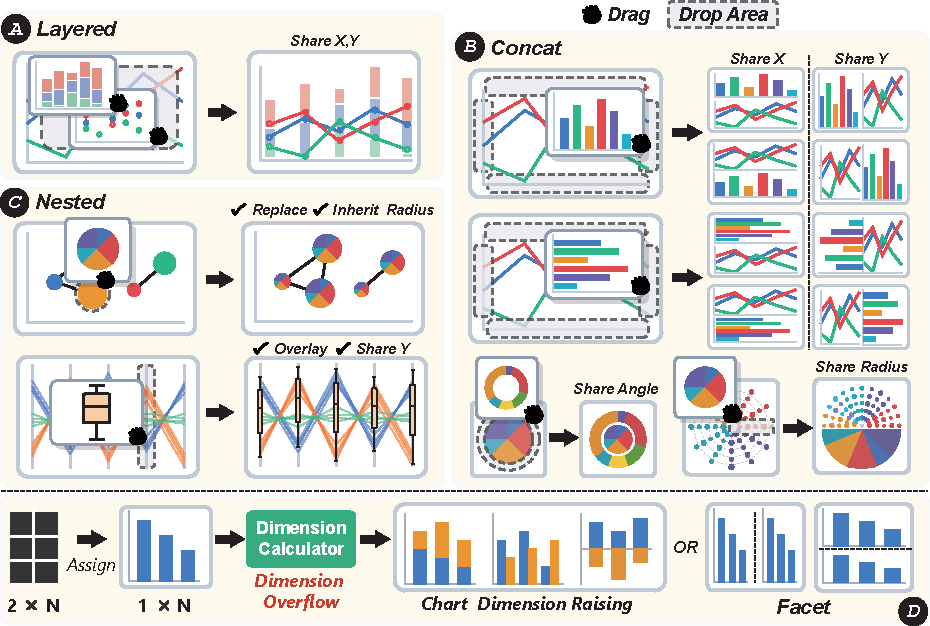
\includegraphics[width=\linewidth]{figs/interaction.pdf}
  \caption{Drag-and-drop interactions for composing chart blocks.
(A) Dropping a block into another block's plotting region creates layering by
sharing both spatial dimensions.
(B) Dropping along a boundary creates concatenation; the boundary determines
the shared dimension and block order. The same interaction extends to polar
coordinates through angular and radial boundaries.
(C) Dropping onto an internal mark or structural element creates nesting,
replacing or overlaying repeated elements while inheriting their data and
spatial references.
}
  \label{fig:drag-drop}
\end{figure*}

\section{CompoVisor}

\subsection{Interaction of Composition}
\label{sec:interaction-design}




{\system} supports composition through both explicit controls and
drag-and-drop, with drag-and-drop serving as the primary interaction for
direct manipulation (Fig.~\ref{fig:drag-drop}). Authors can invoke a
composition operation using dedicated controls or express the same intent
spatially by dragging one block onto a corresponding drop area of another.
During dragging, valid target regions are visualized as drop areas. Each drop
area indicates not only whether the two blocks can be composed, but also the
resulting composition type, shared spatial dimensions, and block ordering.
Dropping outside these regions leaves the blocks independently positioned in
the free-form layout.

\textbf{Identifying composition targets.}
When an author drags one block over another, {\system} highlights valid drop
areas based on their data and coordinate compatibility. Moving across these
areas previews the available composition operations before committing a drop.

\textbf{Layering through an interior drop.}
Dropping a block into the plotting region of another block creates a layered
composition (Fig.~\ref{fig:drag-drop}.A). The two blocks are placed in a common
coordinate space and share both spatial dimensions. For example, dropping a
line chart into the plotting region of a bar chart aligns their $x$ and $y$
encodings and produces a combined bar-and-line visualization. The plotting
region acts as a two-dimensional drop target, distinguishing layering from
blocks that merely overlap in the free-form layout.

\textbf{Concatenation through boundary drops.}
Dropping a block along the boundary of another block creates a concatenated
composition (Fig.~\ref{fig:drag-drop}.B). The selected boundary determines both
the shared dimension and the relative order of the blocks. A drop above or
below the target produces vertical concatenation and shares the $x$ dimension,
whereas a drop to its left or right produces horizontal concatenation and
shares the $y$ dimension. Opposing boundary regions allow authors to determine
which block appears first without invoking a separate reordering command.
The same interaction is interpreted according to the coordinate system of the
participating blocks. In polar coordinates, a radial boundary drop creates
concentric regions that share the angular dimension, while an angular boundary
drop creates adjacent sectors that share the radial dimension. Authors thus
use the same boundary-based gesture across coordinate systems, while the
resulting spatial relationship follows the dimensions of the target
coordinate space.

\begin{figure}[h]
  \centering
  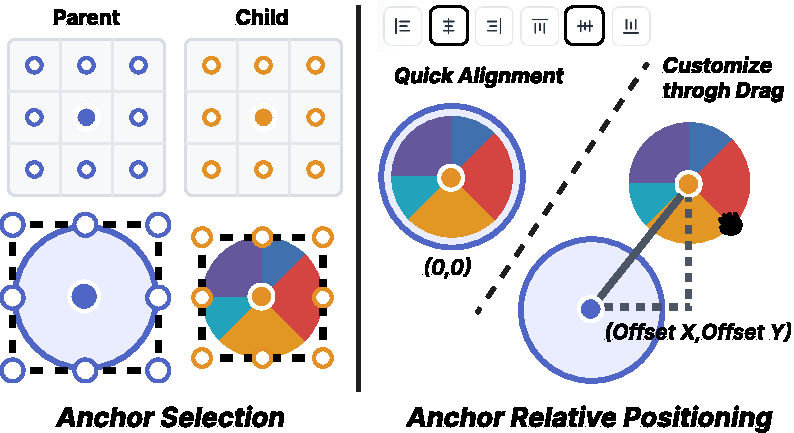
\includegraphics[width=\columnwidth]{figs/nest_anchor_alignment.pdf}
\caption{Anchor-based relative positioning between a parent and child. The selected parent and child anchors define the initial alignment, which can be further refined through direct dragging and an $(x,y)$ offset.}
  \label{nest_anchor_alignment}
\end{figure}

\textbf{Nesting through element-level drops.}
The interaction proceeds from nesting to positioning and composition. First, the author drops a child block onto an eligible mark or structural element (Fig.~\ref{fig:drag-drop}.C), prompting {\system} to associate the child with the corresponding class of parent elements, instantiate it for each eligible element, and establish the required data correspondence. The child is initially aligned to the center of its parent. If further adjustment is needed, the author can open the positioning interface (Fig.~\ref{nest_anchor_alignment}) and independently select an anchor on the parent and the child; then use either quick-alignment presets or drag the child from this anchor-aligned position, with the displacement recorded as an $(x,y)$ offset.



\textbf{Editing composed blocks.}
After a drop is committed, the resulting composition forms a new manipulation
boundary. In the surrounding layout, it behaves as a coherent unit: moving or
resizing the composition preserves the relative positions and shared spatial
relationships of its constituent blocks. To modify these internal
relationships, such as changing the order of concatenated blocks or adjusting
the placement of a nested child, the author enters the composition and edits
its constituent blocks directly. This distinction prevents external layout
operations from inadvertently disrupting an established composition while
retaining access to its internal structure.

\subsection{Compatibility Engine}

The compatibility engine determines whether a dataset can support a
candidate chart type under a given channel assignment. Rather than
reasoning about rendering properties such as marks, axes, or coordinate
systems, the engine focuses exclusively on the data requirements of a
chart. These requirements are represented by a \emph{data contract},
and contract violations are resolved, when possible, through a
\emph{minimal fix}.

\subsubsection{Data Contract}

We describe the data requirements of each chart block using a data contract.
A data contract specifies the required visual channels, the types of fields
that can be assigned to them, and the fields that jointly form the chart key.
An assignment satisfies the contract when each field is compatible with its
channel and the key uniquely identifies the observations required by the
chart. We refer to these two conditions as \emph{type compatibility} and
\emph{key uniqueness}, respectively.

\textbf{Type compatibility.}
Consider a single-line chart whose observations are encoded by horizontal
position \(x\) and vertical position \(y\). Because the \(x\)-channel
determines both horizontal position and connection order, it accepts an
ordered, temporal, or continuous quantitative field. The \(y\)-channel
determines vertical position and therefore requires a quantitative field.
Assigning a nominal field to \(y\), for example, violates type compatibility
because it does not provide the numerical values needed to position
observations vertically. A multiline chart additionally contains a
\emph{series} channel, which partitions observations into separate lines and
therefore requires a discrete field. 


\begin{figure}[h]
  \centering
  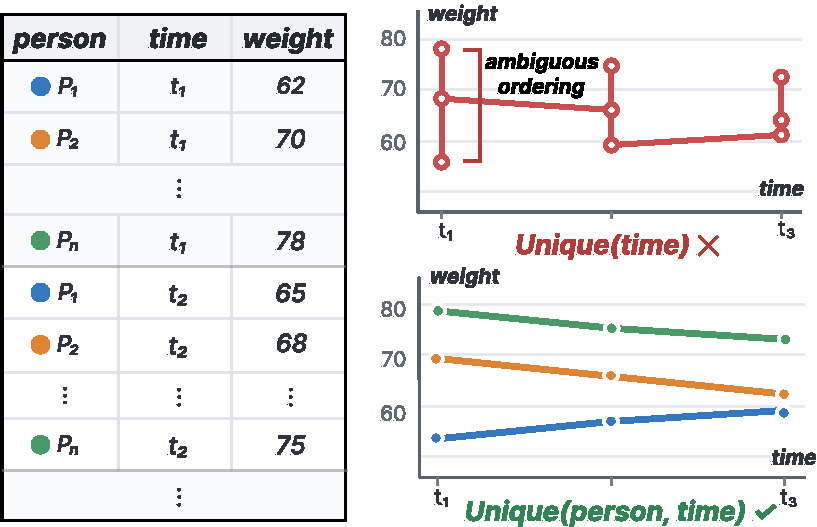
\includegraphics[width=\columnwidth]{figs/unique.pdf}
  \caption{
A single-line chart requires \emph{time} to be unique, which is violated when
multiple people share the same time value. A multi-line chart instead requires
each \((\emph{person}, \emph{time})\) pair to be unique, allowing the
observations to form separate trajectories..}
  \label{fig:data-contract-uniqueness}
\end{figure}

\textbf{Key uniqueness.}
Type compatibility alone does not ensure that the assigned data form a valid
chart. In \autoref{fig:data-contract-uniqueness}, assigning \emph{time} to
the \(x\)-channel and \emph{weight} to the \(y\)-channel satisfies the type
requirements of a single-line chart. However, the data contain one
observation for each person at every time value. Without \emph{person}, these
observations are interpreted as points on the same line. Ordering and
connecting them by \emph{time} introduces vertical segments whose connection
order has no meaningful interpretation. A single-line chart therefore uses
\(x\) as its key and requires each \(x\) value to identify at most one
observation:
\[
    \operatorname{Unique}_{D}(x).
\]
A multiline chart accommodates the same data by assigning \emph{person} to
the series channel. This assignment partitions the observations into
separate trajectories and adds the series field to the key:
\[
    \operatorname{Unique}_{D}(\mathit{series},x).
\]
Neither \(x\) nor series needs to be unique; their combination must identify
each observation. Thus, observations may share an \(x\) value across
different series, but not within the same series unless they are first
aggregated. More generally, a chart key specifies the assigned fields that
must jointly distinguish its observations. Unlike type compatibility, which
can be checked for each channel independently, key uniqueness must be
evaluated jointly over these fields.

\textbf{Contract inheritance in composition.}
Given chart blocks that satisfy their local contracts, composition introduces
additional constraints on how their data and encodings relate across blocks.
\emph{Layering} places blocks in a shared coordinate system and therefore
requires compatibility along both spatial dimensions. Corresponding channels
must have compatible data types and semantics; discrete channels must have
consistent or reconcilable domains, whereas quantitative and temporal
channels must use comparable scales.
\emph{Concatenation} requires compatibility only along the shared coordinate
dimension. Channels on this dimension must have compatible data types,
semantics, domains, and scales, while channels on the partitioned dimension
remain independent.
\emph{Faceting} partitions a block by a discrete field into a finite set of
chart instances. The same contract is applied to each partition so that all
instances maintain a consistent visual structure.
\emph{Nesting} embeds a child block within elements of a parent block. Each
child instance can obtain its input data from the corresponding parent
element, either directly from its bound record or through a shared key that
retrieves related records. The resulting data must provide the fields required
by the child contract. A composition is accepted only when these operator-specific constraints are
satisfied. Otherwise, the composition is disabled until the participating
blocks are configured compatibly.


\subsubsection{Contract Validation and Repair}

Our system validates channel, relational, and composition contracts at
different stages of the authoring workflow. These contracts are used not only
to detect invalid charts, but also to prevent invalid operations and guide
users toward valid alternatives. Channel and composition violations are
mainly prevented through interactive constraints, whereas relational
violations are resolved through explicit repair.

\textbf{Channel contracts} are applied while the user edits a chart block in
the encoding configuration panel. For each visual channel, the contract
specifies its required field type, cardinality, and other role-specific
constraints. The system evaluates the available columns against these
constraints and disables incompatible choices. Invalid channel bindings are
therefore prevented at selection time, rather than detected and repaired
after the chart has been constructed.

\begin{figure*}[t]
  \centering
  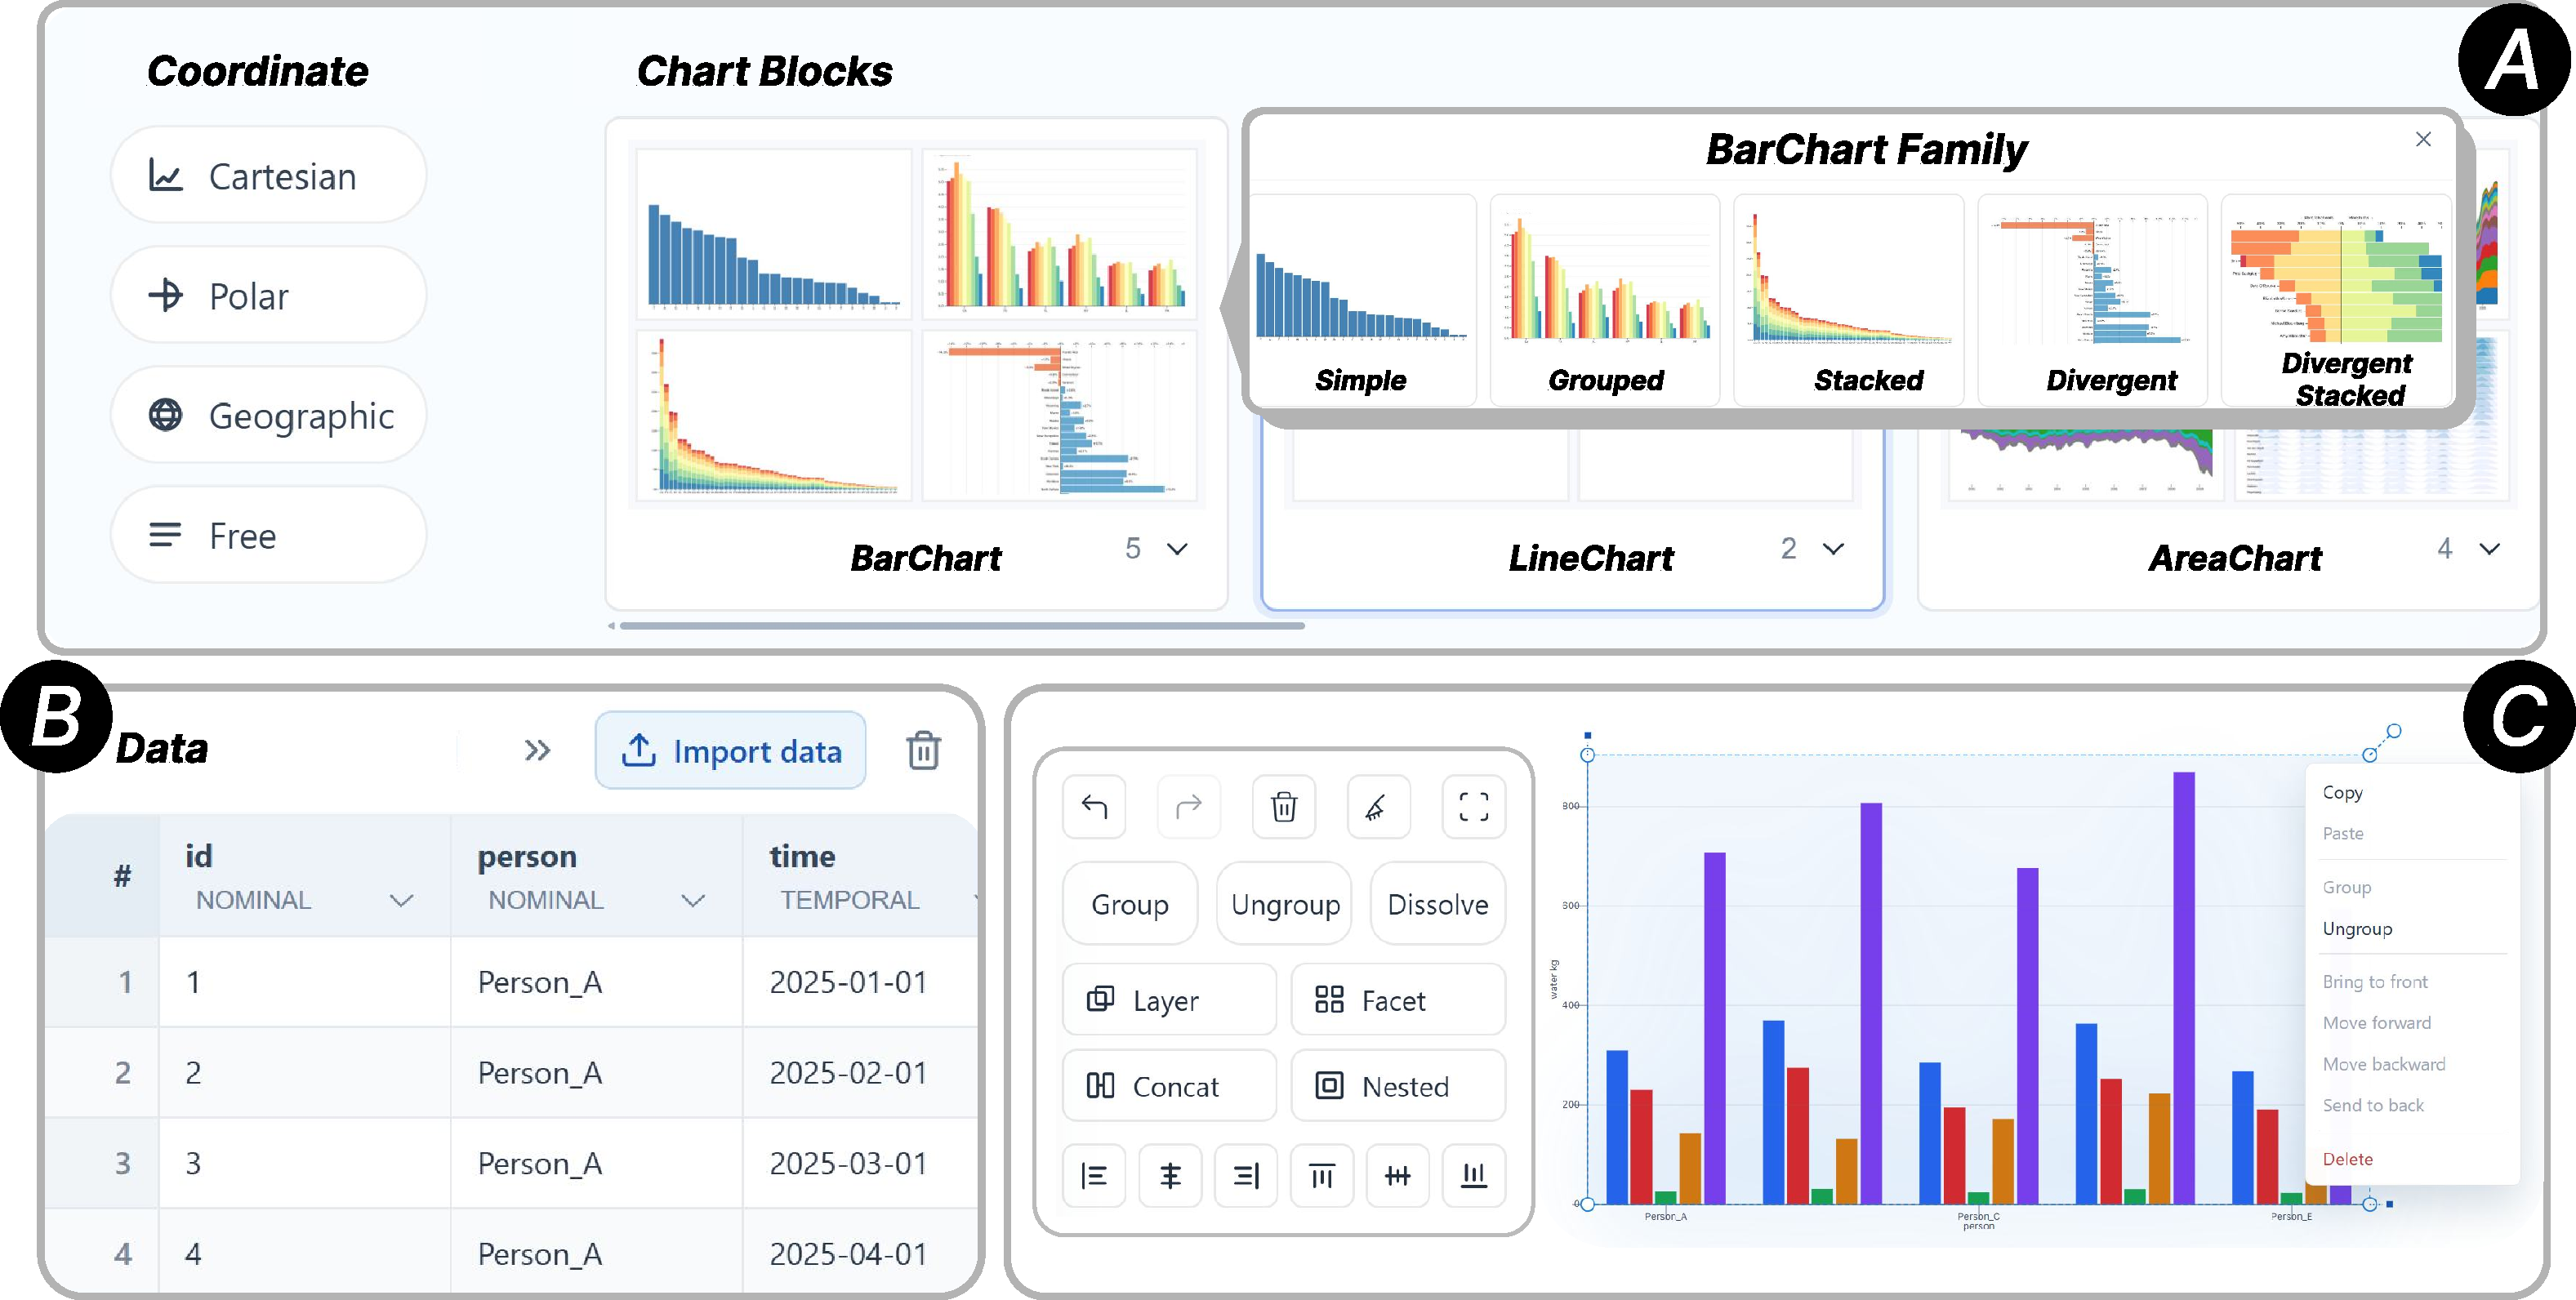
\includegraphics[width=\linewidth]{figs/interface.pdf}
  \caption{interface.
}
  \label{fig:interface}
\end{figure*}

\textbf{Relational contracts} are validated when the user confirms the chart
configuration. The system checks whether the selected visual
dimensions functionally determine the encoded values when such a dependency
is required by the chart contract. If this condition is violated, the system
identifies all inclusion-minimal sets of columns that can distinguish the
conflicting records. A set is inclusion-minimal if none of its proper subsets
can resolve the violation; sets of different sizes are retained as long as
they are independently minimal. The user first selects one candidate set and
then resolves its columns incrementally. For each column, the system offers
three repair strategies: aggregating the conflicting values with an operation
such as sum or mean; introducing the column as an additional visual dimension,
which may upgrade the chart from, for example, a bar chart to a stacked or
grouped bar chart; or using the column to facet the chart. After each repair
operation, the relational contract is revalidated until all conflicts are
resolved.



\textbf{Composition contracts} are used both before and after chart blocks are
composed. Before composition, the system validates the local contracts of the
participating blocks and checks their compatibility according to the selected
composition operator. For example, layering requires compatibility along both
dimensions of the shared coordinate system, whereas concatenation requires
compatibility only along the shared dimension. An incompatible composition is
disabled rather than repaired automatically. Once a composition has been
created, its compatibility constraints are propagated back to the encoding
configuration panels of its constituent blocks. Consequently, editing one
block is constrained by the contracts of the other blocks, and columns that
would invalidate the existing composition become unavailable. 



\subsection{Interface}
\label{sec:interface}


The system is organized as a canvas-based authoring workspace consisting of a
\emph{Block List}, a \emph{Data Panel}, and an \emph{Encoding Config Panel}.

\textbf{Canvas} (\autoref{fig:interface}.C) is the main workspace for arranging and composing chart blocks.
It supports basic editing and layout operations on a zoomable and pannable
board. Chart compositions with drag-and-drop are also performed directly on the Canvas.


\textbf{Block List} (\autoref{fig:interface}.A) is located at the top of the sidebar and provides access
to available chart templates. To reduce the search space, templates are first
filtered by coordinate system: Cartesian, Polar, Geographic, or
coordinate-free. Within each coordinate system, they are grouped into
families such as bar, line, and area. Each family is shown as a compact
preview with representative thumbnails and a template count. Selecting a
family reveals its templates, which can then be dragged onto the canvas and
instantiated as chart blocks.

\textbf{Data Panel} (\autoref{fig:interface}.B) supports importing and inspecting CSV data. Tabular data is
imported as a single CSV file, while graph data is imported as two CSV files,
one for nodes and one for edges. After import, users can preview the data and
adjust the inferred field types to provide appropriate semantics. These types
are then used to check whether fields are compatible with the visual roles of
a chart block.


\textbf{Encoding Config Panel} provides configuration options for the selected
chart block. Using a simplified Vega-Lite-style specification, it allows
users to bind imported data to the block and map data fields to its visual
channels. The available options are determined by the selected chart
template and its encoding requirements. The panel also checks the
compatibility between the data and the chart. When an incompatibility is
detected, it displays the issue and provides applicable resolution options,
such as data aggregation, chart upgrade, or faceting. The configuration can
be confirmed only after all incompatibilities have been resolved.

Together, these components support an iterative workflow: authors import and
inspect data, browse and place a chart block, configure its encodings, arrange
and compose charts on the Canvas, and resolve any remaining structural
incompatibilities through explicit repair choices.








